\documentclass[12pt,fleqn,answers]{exam}
\usepackage{pifont,bbding,url}
\usepackage{dingbat}
\usepackage{amsmath,upgreek}
\usepackage{fleqn}
\usepackage{epsfig}
\usepackage{pdfpages}
\usepackage{mathptm}
\usepackage[activate={true,nocompatibility},final,tracking=true,kerning=true,spacing=true,factor=1100,stretch=10,shrink=10]{microtype}
\usepackage{color}
\usepackage{enumerate}
\usepackage{fourier}
%\usepackage[euler-digits,euler-hat-accent,T1]{eulervm}
\usepackage{amssymb, wasysym, enumerate}
\shadedsolutions
%\definecolor{SolutionColor}{rgb}{0.9,1,1}
\definecolor{SolutionColor}{rgb}{1,1,0.7}
\addpoints
\boxedpoints
\pointsinmargin
\pointname{pts}

\newcommand{\dotprod}{\, {\scriptzcriptztyle \stackrel{\bullet}{{}}}\,}
\begin{document}

\newcommand{\reals}{\mathbf{R}}
\newcommand{\bi}{\mathbf{i}}
\newcommand{\bj}{\mathbf{j}}
\newcommand{\bk}{mathbf{k}}


\newcommand{\ex}{1}
\newenvironment{alphalist}{
  \begin{enumerate}[(a)]
    \addtolength{\itemsep}{-1.0\itemsep}}
  {\end{enumerate}}

\newenvironment{handlist}{
  \begin{enumerate}[\leftthumbsup]
    \addtolength{\itemsep}{-1.0\itemsep}}
  {\end{enumerate}}

\large
\vspace{0.1in}
\noindent\makebox[3.0truein][l]{{\bf MATH 202}}
{\bf Name:}\hrulefill\
\noindent \makebox[3.0truein][l]{\bf In Class work 7}
{\bf Row:}\hrulefill\

\tiny



\begin{questions}

\question The force $F$ required to lift sack of potatoes $x$ feet from the ground level on planet Yavin is
$F(x) = \frac{5}{(1000 + 2 x)^2}$. Find the work done by lifting the sack of potatoes from $x=0$ to $x=1000$.
\begin{solution}[3.0in] 
  For a position dependent force $F$, the work required to move something from
  $a$ to $b$ is $\int_a^b F(x) \,\mathrm{d} x$. So
  \begin{align*}
  \mbox{work} &= \int_0^{1000} \frac{5}{(1000 + 2 x)^2} \, \mathrm{d} x, \\
              &= - \left. \frac{5}{2 (1000 + 2 x)} \right|_{x=0}^{x=1000}, \\
              &= \frac{1}{600}.
  \end{align*}
 
\end{solution}

\question [5] Find the work done moving a $107$ kg mass from $x= -2 $ to $x =5$ if 
the position dependent force is $F(x)= \begin{cases} 5 & x < 1 \\ 8 & x \geq 1 
\end{cases}$, where
the units of force are Newtons and the units of distance are meters.
\begin{solution}[3.0in] 
\begin{align*}
\mbox{work} = \int_{-2}^1 5 \, \mathrm{d}x + \int_{1}^5 8 \, \mathrm{d}x
   = 47.
\end{align*}
\end{solution}

\question[5]  Find the \emph{numerical   value} of  \(\displaystyle  \int_4^7 \frac{1}{3 x - 10} \mathrm{d} x \).   
\begin{solution}%[3.0in]
\[
    \int_4^7 \frac{1}{3 x - 10} \mathrm{d} x = \frac{1}{3}
     \ln\left(\frac{11}{2}\right)
\]
\end{solution}

%\newpage

\question[5] Find a general solution to the DE \(\displaystyle y \frac{\mathrm{d} y}{\mathrm{d} x} = x^2  \).

\begin{solution}[2.5in]
 \[ \frac{1}{2} y^2 =  \frac{1}{3} x^3  + c,\]
 where $c \in \reals$.
\end{solution}

%\newpage


\question Find a formula for each derivative:
\begin{parts}

\part[5]  \(\displaystyle \frac{\mathrm{d}}{\mathrm{d} x} \left( x \mathrm{e}^{-x^2}  \right) \) 
\begin{solution}[1.15in]
  \begin{equation*}
    -\left(\left(2\,x^2-1\right)\,e^ {- x^2 }\right)
  \end{equation*}

\end{solution}

\part[5]  \(\displaystyle \frac{\mathrm{d}}{\mathrm{d} x} \left(\frac{\exp(x) - \exp(-x)}{2} \right) \) 
\begin{solution}[1.15in]
\begin{equation*}
  \frac{\exp(x) + \exp(-x)}{2}
\end{equation*}
\end{solution}
\part[5]  \(\displaystyle \frac{\mathrm{d}}{\mathrm{d} x} \left( x  \ln(x) \right) \) 
\begin{solution}[1.15in]
\[
1 + \ln(x).
\]
\end{solution}

\part   \(\displaystyle \frac{\mathrm{d}}{\mathrm{d} x}  \ln \left(\frac{1+x}{1-x}\right)$

\begin{solution}[1.15in]
\[
\frac{2}{{1-{x}^{2}}}.
\]
\end{solution}


\end{parts}

\question [5] Find the numerical value of $\int_{1}^2 1 + \ln(x) \, \mathrm{d} x$.  \textbf{Hint:} Look at your answer to part `c' of the previous question.
\begin{solution}[2.5in]
\[2 \log{(2)}\].
\end{solution}
%\newpage

\question Let \(Q\) be the portion of the \(x y\) plane described by \(0 \leq x \leq 1 \) and \(0  \leq y \leq 1 - | x - 1| \).


\begin{parts}

\part [5] Draw a nicely \emph{labeled} picture of the set \(Q\).

\begin{solution}[2.5in] 

\centering
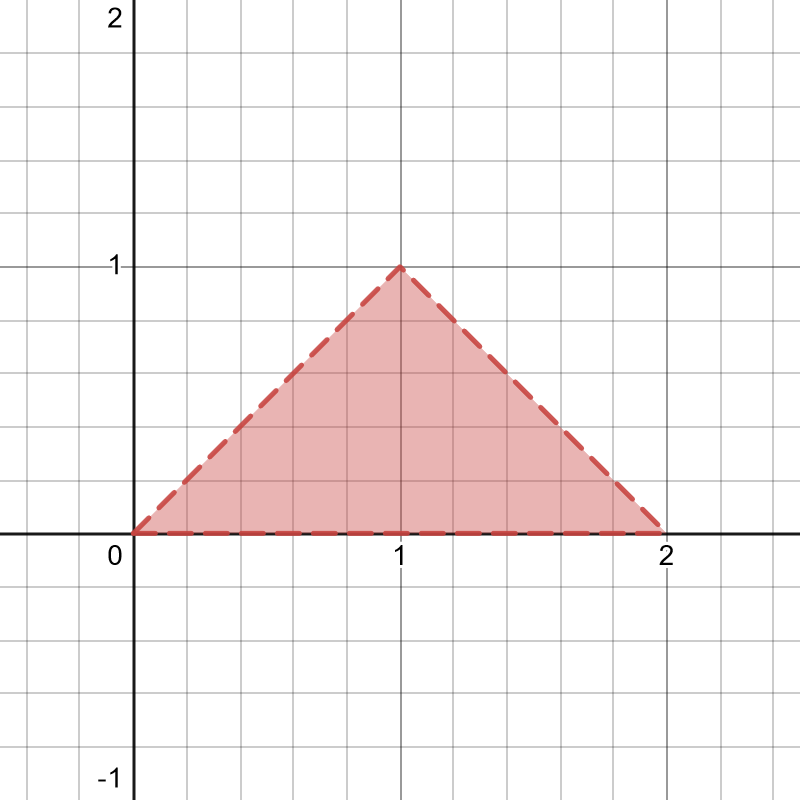
\includegraphics[scale=0.25]{desmos-graph(56)}

\end{solution}

%\newpage

\part [5] Using \emph{disks} (that is strips \emph{perpendicular} to the axis of rotation), find the \emph{volume}
of the solid generated by rotating \(Q\) about the \(x\) axis. Express the result as a \emph{definite integral}, but
\textbf{do not} find the numerical value of the definite integral.

\begin{solution}[2.5in] 
\[
   \uppi \int_0^1  \left(1 - |x-1|\right)^2  \, \mathrm{d} x.
\]
\end{solution}

%\newpage
\part [5] Using \emph{shells} (that is, strips \emph{parallel} to the axis of rotation), find the \emph{volume}
of the solid generated by rotating \(Q\) about the \(x\) axis. Express the result as a \emph{definite integral}, but
\textbf{do not} find the numerical value of the definite integral.


\begin{solution}[2.5in] 
To find the length of the strip, we need to solve $y = 1 - |x-1|$
for $x$. The solutions are $x = y$ and $x=2 - y$. The length of
the strip is $2-y - y$ or $2 - 2 y$.
\[
   2 \uppi \int_0^{2}  y  (2-2 y)  \, \mathrm{d} y.
\]
\end{solution}

\part [5] Using a strip that is parallel to the $y$ axis, find area of $Q$.

\begin{solution}[2.5in] 
  \begin{equation}
    \int_0^{1}    (2-2 y)  \, \mathrm{d} y = 1.
\end{equation}

\end{solution}

%\newpage
\part [5] Using a strip that is parallel to the $y$ axis, find the $y$ coordinate of the centroid of $Q$.

\begin{solution}[2.5in] 
  \begin{equation}
    \mbox{Area}  \times \overline{y} = \int_0^1 y   (2-2 y) \, \mathrm{d} y 
     = \frac{1}{3}.
   \end{equation}
   Since the area is one, $\overline{y} = \frac{1}{3}$.
\end{solution}

\part [5] Using a strip that is parallel to the $y$ axis, find the $x$ coordinate of the centroid of $Q$.

\begin{solution}[2.5in] 

  \begin{equation}
    \mbox{Area} \times  \overline{x} =  \frac{1}{2} \int_0^1 \left( (2-y)^2 - y^2 \right) \, \mathrm{d} y
    = 1.
   \end{equation}
\end{solution}
\end{parts}

\question[5] Express the arclength of the portion of the curve $y = x^2$ 
with $-1 \leq x \leq 1$. Do not
attempt to find the numerical value of the definite integral.
\begin{solution}[2.5in]
\[ \int_{-1}^1 \sqrt{1 + 4 x^2} \, \mathrm{d} x\]
\end{solution}


%\newpage
\question [5] Show that $y^5=x+ c$ is a general solution to the DE $y^4  \frac{\mathrm{d} y}{\mathrm{d} x}  = 1/5$.

\begin{solution} Differentiating $y^5=x+ c$ gives 
  $5 y^4 \frac{\mathrm{d} y}{\mathrm{d} x} = 1$. Dividing that by
  $5$ yields the given DE.

\end{solution}
\end{questions}
%\includepdf[pages={1-}]{cheat_sheet.pdf}     
\end{document}